\begin{figure*}[b]
	\centering
	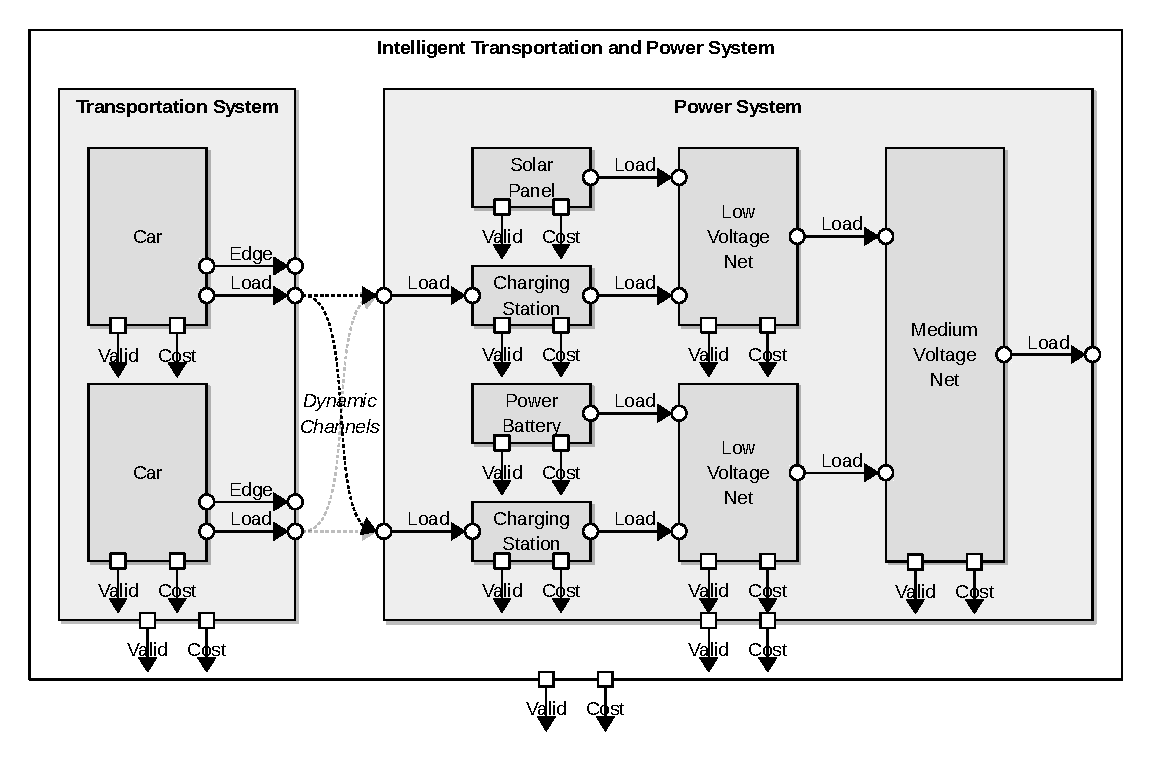
\includegraphics[width=\textwidth]{../gfx/model.pdf}
	\caption{Overview of the holistic modeling approach including transportation and power system connected by dynamic channels.}
	\label{fig:model}
\end{figure*}

\section{Transportation and power systems modeling}
\label{section:contribution}

Based on the underlying systems modeling technique (see Sec.~\ref{section:foundation}), we propose an integrated transportation and power system model as shown in Figure~\ref{fig:model}. At its root, the model defines an intelligent transportation and power system component, which contains separate components for the transportation and the power system. The transportation system component comprises the individual car components traveling along the traffic infrastructure. Similarly, the power system component includes the individual electric components, such as static loads, solar panels, power batteries and charging stations as well as electric infrastructure consisting of low-voltage and medium-voltage net components. 
%aComponents can be instantiated with specific configurations. 
%Subsequently we describe the different components of the model in terms of their ports, channels and behavior.

\subsubsection*{Intelligent transportation and power system (IS)}
\label{section:intelligent_system}

The $IS$ contains the transportation system $TS$ and the power system $PS$. The $IS$ defines dynamic channels between the car load outputs of the $TS$ and the charging station load inputs of $PS$. Consequently, each car is connected to each charging station statically, but loads are forwarded only to the connected charging station dynamically. Therefore, the dynamic channel conditions test whether a dynamic car position matches a static charging station position. Furthermore, the $IS$ specifies a cost output which aggregates the cost of the $TS$ and the $PS$ using their individual weights. On this cost output a minimization objective is defined through annotation. 
%Finally, no additional constraints are defined on system state and behavior.

\subsubsection*{Transportation system (TS)}

The $TS$ comprises the traffic infrastructure $TN$ as well as the car components $C$. The $TN$ is modeled as directed graph $G = (V,E)$ with nodes $V$ and edges $E \subseteq V \times V$. Here, nodes $v,w \in V$ represent reference points in $TN$ such as intersections. Nodes define an absolute position in real-world coordinates (latitude, longitude and elevation): 
%(i.e. latitude,longitude, and elevation):
$$\mathit{latitude}: V \to \mathbb{R}_0^+$$ 
$$\mathit{longitude}: V \to \mathbb{R}_0^+$$ 
$$\mathit{elevation}: V \to \mathbb{R}_0^+$$ 
In contrast, edges $(v,w) \in E$ represent road segments between source nodes $v$ and target nodes $w$ with a defined number of lanes as well as road type (e.g.\ residential streets or stations). Finally, the $TS$ defines a cost output which aggregates the cost of the individual cars $C$. To ensure valid behavior, the $TS$ implements a constraint over the car positions which calculates the largest number of pair-wise overlapping cars per segment $(v,w) \in E$ and compares it to the available number of lanes.

\subsubsection*{Car (C)}
\label{section:car}

%atomic components in our system model and are defined in terms of a range of parameters.
$C$ represent entities on the traffic infrastructure, whose basic physical properties are length and weight: 
$$\mathit{length}: C \to \mathbb{R}_0^+$$ 
$$\mathit{weight}: C \to \mathbb{R}_0^+$$ 
When it's departure time (a specific time point) has passed during simulation, the $C$ starts traveling from its origin to a specified destination position. Origin, destination and position of $C$ are edges $(v,w) \in E$ of the traffic infrastructure $TN$. The distance between two nodes, i.e. the length of an edge is defined as
$$\mathit{distance}: V \times V \to\mathbb{R}_0^+$$ 
When starting to travel, the position of a $C$ equals the origin, while subsequent positions are selected from a set of possible routes. The set of possible routes equals the $k \in \mathbb{N}$ shortest paths from the position to the destination position or the nearest charging station. Of these alternatives one route is selected randomly. The current position consists of the current edge and traveled distance on this edge.
$$\mathit{position} = \{(e,d): E \times \mathbb{R}_0^+ \}$$ 
with $e = (v,w)$ such that $d \leq distance(v,w)$.
%depending on a selection probability parameter. If the state of charge falls below a specified percentage, route selection probability shifts towards preferring the nearest charging station. 
$C$ contain a battery with a state of charge (SOC) and a defined capacity to which the $C$'s energy consumption and production are applied to.
Energy consumption occurs during driving along the $TN$ or during discharge at charging stations. While driving, energy consumption is based on the $C$'s energy efficiency, traveled elevation profile (slope), weight as well as the randomly selected speed (limited to a maximum) in each simulation step. Slope is defined as:
$$\mathit{slope} : V \times V \to \mathbb{R}_0$$ 
$$\mathit{slope(v,w)} = \frac{distance(v,w)}{elevation(w)-elevation(v)}$$ 
Energy production occurs during driving (i.e.\ energy recuperation) or during charging at charging stations. To ensure valid behavior, a constraint tests whether the SOC lies within a constant minimum and maximum. When connected to a charging station, a charging mode is chosen probabilistically with uniform distribution. If the $C$ chooses charging, a load is transferred from the charging station to the $C$. If the $C$ chooses discharging, a load is transferred from the $C$ to the charging station instead. Furthermore, the $C$ can choose an idle state.
% mode transferring no power load. The speed of charging and discharging is subject to a defined charge rate. 
Finally, the $C$ objective includes multiple cost factors.
%after its departure time has passed. 
The first cost factor evaluates the $C$'s state of charge with respect to the $C$'s maximum state of charge. The second cost factor aggregates the time needed to reach its specified destination position. The third cost factor measures the energy consumption in relation to the maximum energy consumption. Then, the cost factors are aggregated and weighted using the weights of the individual cost factors.

\subsubsection*{Power system (PS)}

The $PS$ represents the overall electric infrastructure including individual electric devices as well as low-voltage nets $LV$ and medium-voltage nets $MV$ (higher voltage nets are omitted currently). Currently supported devices include static loads $SL$, solar panels $SP$, power batteries $PB$ and charging stations $CS$. At its interface the $PS$ specifies a cost output that aggregates the cost of the electric infrastructure and it's devices.
%In principle, different aggregation schemes can be used. 
The $PS$ forwards the load of the medium-voltage net representing the final load balance.

\subsubsection*{Low/medium-voltage nets (LV/MV)}

$LV$/$MV$ receive loads from connected electric devices and provide an aggregate load output to the upper voltage level. Note that connected electric devices can be $LV$ as well. 
%During simulation, low-voltage nets sum up the loads of all connected electric devices to yield the load output. 
%The medium-voltage net aggregates the loads of all low-voltage nets instead. 
Based on the aggregated load, a net's cost output is specified relative to the total net capacity (i.e.\ the closer to the capacity, the worse). Then, each net's cost output is dampened based on a defined weight. Finally, to ensure valid behavior a constraint tests if a net's aggregated load as well as all connected loads lie within the net's total capacity. More information on the model can be found in~\cite{hackenberg2012applying}.

\subsubsection*{Static load (SL)}

$SL$ aggregate a wide range of electric devices, which cause non-controllable loads (such as conventional light bulbs or washing machines). Consequently, they abstract from specific details about different electric devices, i.e. producers and consumers, reducing the available information to their load per time instant only. The result of this aggregation is defined in terms of a load profile $L = (l_t)_{0 \leq t \leq n}$ with $t,n \in \mathbb{N}$ representing current and maximum time points and $l_t \in \mathbb{R}$ representing positive or negative loads.
%with unit kW/h. 
%To vary static (i.e.\ non-controllable) load in different scenarios easily, 
Furthermore, a defined scale factor may dampen the static profile. 

\subsubsection*{Power battery (PB)}

$PB$ represent stationary electric devices acting as both producers and consumers (e.g.\ lead-acid batteries). 
%In each simulation step, $PB$ choose randomly between charging, discharging or idle mode with selection of modes being uniformly distributed. 
Depending on random selection of a mode in each simulation step, energy consumption (i.e.\ negative load) or production (i.e.\ positive load) can be observed on the low-voltage net side. Production and consumption are subject to a defined charge rate and affect the state of charge (SOC) of the $PB$ which has a specified capacity.
%Charging is subject to the battery's energy conversion effectiveness, while the SOC is subject to energy loss over time. 
To ensure valid behavior, a constraint tests whether the SOC lies within a constant minimum and maximum. Detailed information about the model can be found in~\cite{hackenberg2014rapid}.

\subsubsection*{Solar panel (SP)}

$SP$ are electric devices which represent one class of renewable energy producers with a defined yield. Based on a specific power scale, $SP$ produce a positive load peaking at the mean time point with a specified variance. Moreover, based on uniformly distributed probabilistic selection $SP$ can choose to dampen their production (known as maximum power point tracking). Detailed information about the model can be found in~\cite{hackenberg2014rapid}.

\subsubsection*{Charging station (CS)}
\label{section:charging_station}

$CS$ represent electric devices acting as consumers or producers and interacting with the cars $C$ of the transportation system $TS$. They are assigned a physical location, i.e.\ an edge $(v,v) \in E$ of the traffic network $TN$ with zero length (i.e.\ same source and target node $v \in V$):
$$\mathit{position}: CS \to E$$ 
 Based on dynamic connection to the cars, $CS$ behavior is determined by the selected charging mode of the currently connected car $C$. 
 %Here, a $CS$ can exhibit zero, negative or positive load on the low-voltage net side. 
 When a load is transferred from the $CS$ to the car, energy consumption can be observed on the low-voltage net side. In contrast, when a load is transferred from the car to the $CS$, energy production can be observed. Transfer rates are subject to a specific charge rate.